% !TEX TS-program = xelatex
% !TEX encoding = UTF-8 Unicode
% !Mode:: "TeX:UTF-8"

\documentclass{resume}
\usepackage{zh_CN-Adobefonts_external} % Simplified Chinese Support using external fonts (./fonts/zh_CN-Adobe/)
% \usepackage{NotoSansSC_external}
% \usepackage{NotoSerifCJKsc_external}
% \usepackage{zh_CN-Adobefonts_internal} % Simplified Chinese Support using system fonts
\usepackage{linespacing_fix} % disable extra space before next section
\usepackage{cite}
\usepackage{tabu}
\usepackage{progressbar}
\usepackage{multirow}

\begin{document}
\pagenumbering{gobble} % suppress displaying page number
\Large{
  \begin{tabu}{ c l r }
    \multirow{4}{1in}{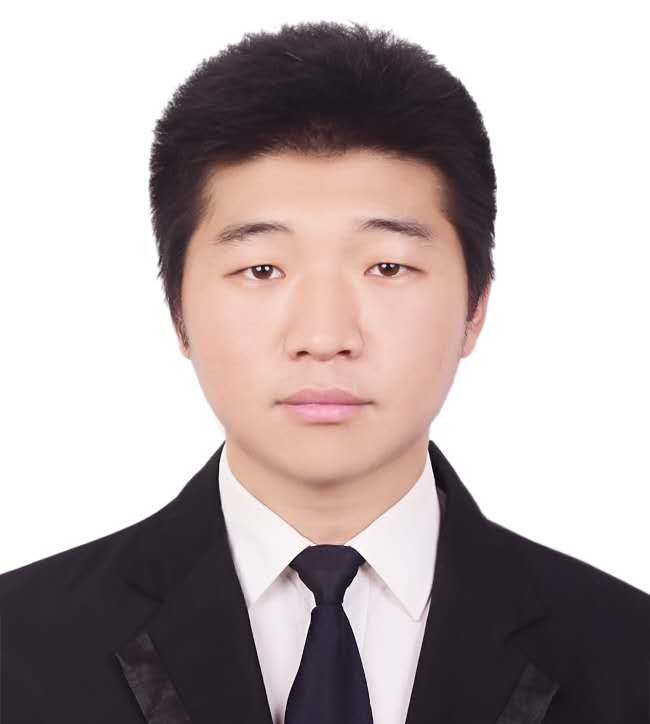
\includegraphics[width=1in]{profile}} & \scshape{Gao Yahu} & {Linux~}\progressbar{0.90} \\
    & \email{gao\_yahu@163.com} & {Python~}\progressbar{0.89} \\
    & \phone{(+86) 131-2029-0626\ \ \ \ } & {C~}\progressbar{0.90} \\
    & \github[github.com/yahugao]{https://github.com/yahugao} & {shell~}\progressbar{0.85}
  \end{tabu}
}
\section{\faCogs\ Knowledge \& Skills}\normalsize
\begin{itemize}
\item {Know all about the skill of Linux system and its common debugging methods, master the technology of the file system in Linux system.}
\item {Know all about the skill of Yocto which used to build Linux distribution. Extensive adapting recipe experiences in building WindRiver Linux.}
\item {Extensive debug experiences in user-mode of QEMU and virtualization of process.}
\item {Extensive operation experiences in Git, Vim and Emacs.}
\item {Familiar with CVE. Expert on fixing CVE via backporting patch from upstream for relevant software.}
\item {Hands-on experiences in building RPM package. Familiar with maintain the SPEC file of RPM package.}
  \item {Knowledge of JAVA, C++, Go, Android and Latex.}
  \end{itemize}

\section{\faUsers\ Experience}\normalsize
\datedsubsection{\textbf{CIeNET Technologies}, Beijing}{Sep. 2017 -- Nov. 2019}
\role{Linux Engineer}{Duty: Maintain WindRiver linux system}
\begin{itemize}
\item Participated in maintaining and testing the WindRiver Linux System, communicated with customer about project requirement. Investigate and fix issues exported during system running. I worked on:
  \begin{itemize}
    \item Fix CVEs released on NVD site and affecting WindRiver Linux system.
    \item Investigate the issues exported by the customers during using WindRiver Linux system and fix them.
    \item Investigate and fix the bad case caused by upgrading.
    \item Integrate software with specific version as customer's requests.
      \item Build Management System for Git repositories.
    \end{itemize}

  \end{itemize}

% \end{itemize}

% \section{\faUsers\ 实习经历}\normalsize
\datedsubsection{\textbf{Intel (China) Co. Ltd},Beijing}{Aug. 2016 -- Feb. 2017}
\role{Engineer Intern}{Duty: Port and verify LTP(Linux test project) from PC to mobile client}
\begin{itemize}
\item Major engineer of porting LTP cross operation system. Worked on:
  \begin{itemize}
  \item Enable LTP on Android system.
  \item Fix bugs caused by different platform.
  \item Push common patches to upstream of LTP.
  \end{itemize}
\end{itemize}

\section{\faGraduationCap\  Education}\normalsize
\datedsubsection{\textbf{The PLA Information Engineering University}, zhengzhou, Henan}{Sep. 2014 -- Jul. 2017}
\textit{Master} in Computer sience and technology (CS)
%\role{硕士研究生}{专业:计算机科学与技术 方向:软件分析与逆向工程}
\begin{itemize}
\item Research how to improve the performance of dynamic binary translation system. Worked on:
  \begin{itemize}
  \item Design and implement retrieving library function locally during dynamic translation
  \item Design and implement translation math library file cross architecture.
  \item Implement retrieving translated math library file during dynamic translation.
  \end{itemize}

\end{itemize}
\datedsubsection{\textbf{Hebei Polytechnic University}, Tangshan, Hebei}{Sep. 2010 -- Jul. 2014}
\textit{B.S} in Computer sience and technology (CS)

%\datedsubsection{\textbf{\LaTeX\ 简历模板}}{2015 年5月 -- 至今}
%\role{\LaTeX, Python}{个人项目}
%\begin{onehalfspacing}
%优雅的 \LaTeX\ 简历模板, https://github.com/billryan/resume
%\begin{itemize}
%  \item 容易定制和扩展
%  \item 完善的 Unicode 字体支持,使用 \XeLaTeX\ 编译
%  \item 支持 FontAwesome 4.5.0
%\end{itemize}
%\end{onehalfspacing}

% Reference Test
%\datedsubsection{\textbf{Paper Title\cite{zaharia2012resilient}}}{May. 2015}
%An xxx optimized for xxx\cite{verma2015large}
%\begin{itemize}
%  \item main contribution
%\end{itemize}


% \section{\faCogs\ IT 技能}\normalsize
% increase linespacing [parsep=0.5ex]
%\begin{itemize}[parsep=0.5ex]
%  \item {编程语言: C == Python > Java > C++}
%  \item 平台: Linux
%  \item 工具: Yocto,rpm,vim
%\end{itemize}
%\datedsubsection{\textbf{COURSERA 认证}}{2018年10月}
%\begin{itemize}[parsep=0.5ex]
%	\item 证书名称: Machine Learning
%	\item 证书编号: NFCZEBTZ5T4L
%	\item 证书URL : https://www.coursera.org/account/accomplishments/verify/NFCZEBTZ5T4L
%\end{itemize}


%\section{\faHeartO\ 获奖情况}
%\datedline{\textit{第一名}, xxx 比赛}{2013 年6 月}
%\datedline{其他奖项}{2015}

\section{\faInfo\  Miscellaneous}\normalsize
% increase linespacing [parsep=0.5ex]
\begin{itemize}
\item {Hobbies: Running, Swimming.}
\item{Participated competition of Named Entity Recognition on Tianchi, TOP100 in 2,000 teams.}
\item {\href{https://www.coursera.org/account/accomplishments/verify/NFCZEBTZ5T4L}{Get Coursera certification of Machine Learning.} }
\end{itemize}

%% Reference
%\newpage
%\bibliographystyle{IEEETran}
%\bibliography{mycite}
\end{document}

%%% Local Variables:
%%% mode: latex
%%% TeX-master: t
%%% End:
